% Instructions to change to html version:
% Comment out:
%  minipage, multicols,columnbreak, mathbf, hrule
% Replace all: \begin{minipage}% \end{minipage} %\begin{multicols}  %\end{multicols}  %\columnbreak % \begin{framed} %\end{framed} %\hrule
% Search for \mathbf
% Replace $$ with \[ and $ with \(
% Enclose graphics in figure environments and add captions:
% Search for  \includegraphics
% Re-tag \df environments as sections, subsections, etc.
% Command Line Code to Create html version:
%First: pdflatex -shell-escape filename.tex                                   
%Second, for each figure: inkscape "filename-figure1.pdf" -o "filename-figure1.png"
% Third: htlatex filename.tex "ht5mjlatex.cfg, charset=utf-8" " -cunihtf -utf8"
\documentclass[10pt]{article}

%\usepackage{tikz, pgf,pgfplots,wasysym,array}
%\usepackage{wasysym,array}

\usepackage{amsmath,amssymb}

\ifdefined\HCode
  \def\pgfsysdriver{pgfsys-tex4ht-updated.def}
\fi 
%\ifdefined\HCode
%  \def\pgfsysdriver{pgfsys-dvisvgm4ht.def}
%\fi 
\usepackage{tikz}
\usetikzlibrary{calc,decorations.markings,arrows}
\usepackage{pgfplots}

\pgfplotsset{compat=1.12}
\usepackage{myexternalize}
\usetikzlibrary{calc,decorations.markings,arrows}
\usepackage{framed}
\usepackage[none]{hyphenat}

\input{../../../common/1336_header_test.tex}
% \input{header.tex}

\usepackage{multirow, array}
\begin{document}

\everymath{\displaystyle}



\newcommand{\ihat}{\boldsymbol{\hat{\textbf{\i}}}}
\newcommand{\jhat}{\boldsymbol{\hat{\textbf{\j}}}}
\newcommand{\khat}{\boldsymbol{\hat{\textbf{k}}}}

\let\oldvec\vec
\renewcommand{\vec}[1]{\oldvec{\boldsymbol{#1}}}

\renewcommand{\u}{\vec{u}}
\renewcommand{\v}{\vec{v}}
\newcommand{\w}{\vec{w}}
\renewcommand{\r}{\vec{r}}
\renewcommand{\a}{\vec{a}}
\renewcommand{\b}{\vec{b}}

\newcommand{\<}{\left\langle}
\renewcommand{\>}{\right\rangle}

\renewcommand{\myTitle}{MATH 1336: Calculus III}

\renewcommand{\mySubTitle}{Sections 2.1 \& 2.2:  Intro to Vectors\\ \& Three Dimensional Coordinate Systems
}
%~\hfill Name: \underline{~~~~~~~~~~~~~~~~~~~~~~~~~~~~~~~~~~~~~~~~~~~~~~~}

\lectTitle{\vspace*{-.5in}\myTitle}{\vspace*{.1in}\mySubTitle \vspace*{-.25in}}

\rfoot{{\texttt{Page \thepage~of \pageref{lastpage}}}}


\setlength{\columnseprule}{0.4pt}
\setlength{\columnsep}{3em}

%\hspace*{-.8in}\begin{minipage}{1.25\textwidth}
%\begin{framed}

\section*{Three Dimensional Coordinate Systems:}




%\begin{minipage}{.4\textwidth}



\begin{figure}[!h]
\centering
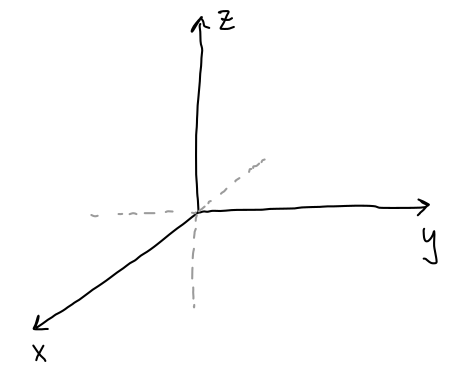
\includegraphics[height=2.in]{3D-axes.png}
\caption{Drawing of a set of 3D coordinate axes in the standard orientation.}
\end{figure}


%\end{minipage}
\hspace*{.2in}
%\begin{minipage}{.5\textwidth}


%\textbf{New Vocabulary:} \\
To describe the position of a point in three dimensional space, we need three coordinate axes: the \(x-\)axis, \(y-\)axis, and \(z-\) axis.\\
 A point \(P\) with coordinates \(x=a,\ y=b,\ z=c\), is described using an ordered triple, \(P: (a,b,c)\).\\~\\
 
 \textbf{Distance Formula:} To find the distance between two points, \(P_1\) and \(P_2\), use:\\
\[
|P_1 P_2| = \sqrt{(\Delta x)^2 + (\Delta y)^2 +(\Delta z)^2}
\]

~\\
A \textbf{cylinder} is a surface that consists of all lines that are parallel to a given line and pass through a given plane curve.\\~\\



%\vspace*{-.2in}
%\end{minipage}

%\end{framed}
%\end{minipage}

%\begin{framed}
%\textbf{New Vocabulary:} \\
%A \textbf{cylinder} is a surface that consists of all lines that are parallel to a given line and pass through a given plane curve.\\~\\
%\textbf{Distance Formula:} To find the distance between two points, \(P_1\) and \(P_2\), use:\\
%\[
%|P_1 P_2| = \sqrt{(\Delta x)^2 + (\Delta y)^2 +(\Delta z)^2}
%\]
%
%\end{framed}
\section*{Example 1:}
Let's get some practice visualizing surfaces in 3D!

Draw, and describe in words,  the surfaces described by the following equations.\\
\textit{Hint:}  Start by sketching cross-sections in the relevant coordinate plane.\\

%\begin{multicols}{2}
\begin{enumerate}[(a)]


\item \(\qquad y=6\)
\vspace*{1.5in}

\item \(\qquad y = x\)
\vspace*{1.5in}

\item \(\qquad x^2 + y^2 = 1\)
\vspace*{1.5in}

\item \(\qquad 1 \leq x^2 + y^2 + z^2 \leq 4, \qquad z \geq 0\)
\vspace*{1.5in}




\end{enumerate}

%\end{multicols}



\section*{Problems for Group Work:}

\begin{enumerate}[{Problem }1]

\item Calculate the distance from \(P_1: (4, -2, 6)\) to each of the following:
\begin{enumerate}
\item The origin
\item The point \(P_2: (1,1,0)\)
\item The \(xy-\)plane
\end{enumerate}

\vfill

\item Draw, and describe in words,  the surfaces described by the following equations.\\
\textit{Hint:}  Start by sketching cross-sections in the relevant coordinate plane.\\



\begin{enumerate}


\item \(\qquad x^2+y^2 = 3^2\)

\item \(\qquad y^2+z^2 = 1\)

\item \(\qquad z=y^2\)

\item \(\qquad xy=1\)

\item \(\qquad x^2+y^2 =z^2\)


\end{enumerate}

\vfill
\end{enumerate}

\pagebreak
%\section*{Intro to Vectors:}

%\hspace*{-.8in}\begin{minipage}{1.25\textwidth}
%\begin{framed}

\section*{Intro to Vectors:}




%\begin{minipage}{.4\textwidth}



\begin{figure}[!h]
\centering
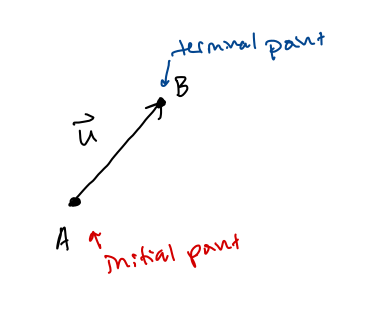
\includegraphics[height=2.5in]{vector-intro.png}
\caption{Illustration of a vector with initial point A and terminal point B.}

\end{figure}


%\end{minipage}
\hspace*{.2in}
%\begin{minipage}{.5\textwidth}
%\textbf{Vocabulary:} \\~\\
A \textbf{scalar} is a quantity that that is fully described by a magnitude (numerical value) alone.\\
\textit{ Example:} -5\\~\\
A \textbf{vector} is a quantity that is fully described by both a magnitude and a direction.\\
\textit{ Example: }\(\v = \<2,-3,7\> = 2\ihat -3\jhat+7\khat\)
 \\~\\
To find the \textbf{magnitude} (length) of a vector, use the same idea as the distance formula. If \(\a=\<a_1,a_2,a_3\>\), then the length of \(\a\) is:
\[
||\a|| = \sqrt{a_1^2+a_2^2+a_3^2}
\]
~\\
A vector with length one is called a \textbf{unit vector}. \\
A ``hat'' instead of an arrow over a vector denotes that it has unit length:
\[
\hat{\boldsymbol{a}} = \frac{\a}{||\a||}
\]
%\end{minipage}

%\end{framed}
%\end{minipage}
\section*{Vector Practice:}


\begin{enumerate}
\item Some of the following quantities are vectors, and some are scalars. Classify them all by checking the appropriate box, and come up with two or three others with which to stump your classmates, and hopefully your instructor.
\begin{center}
\large
\begin{tabular}{|l|c|c|}
\hline
\textbf{Quantity}&\textbf{Vector?}&\textbf{Scalar?}\\ \hline
Speed&&\\ \hline
Force&&\\ \hline
Bank Account Balance&& \\ \hline
Velocity &&\\ \hline
Acceleration&& \\ \hline
Energy &&\\ \hline
Temperature&& \\ \hline
Work &&\\ \hline
Electrical Current &&\\ \hline
\end{tabular}
\end{center}
\vfill

\item Calculate the following quantities, given the vectors listed below.
\label{lastpage}
\[
\u=\<8,0,0\>, \qquad \v = 5\ihat+5\jhat, \qquad\a=\<-1,1,1\>, \qquad\b=\<1,2,3\>
\]
%\begin{multicols}{2}
\begin{enumerate}
\item \(3\v\)
\item \(\a+\b\)
\item \(||\b||\)
\item \(||\u||\)
\item \(\u+\v\)
\item Find a unit vector that points in the same direction as \(\u\)
\item Find a unit vector that points in the opposite direction from \(\a\)
\end{enumerate}
%\end{multicols}
\end{enumerate}

%\label{lastpage}

%\pagebreak

\end{document}
